% Editable native annotations around unchanged verified IDE photographs.
\par
\begin{figure}[htbp]
\centering
\sbox0{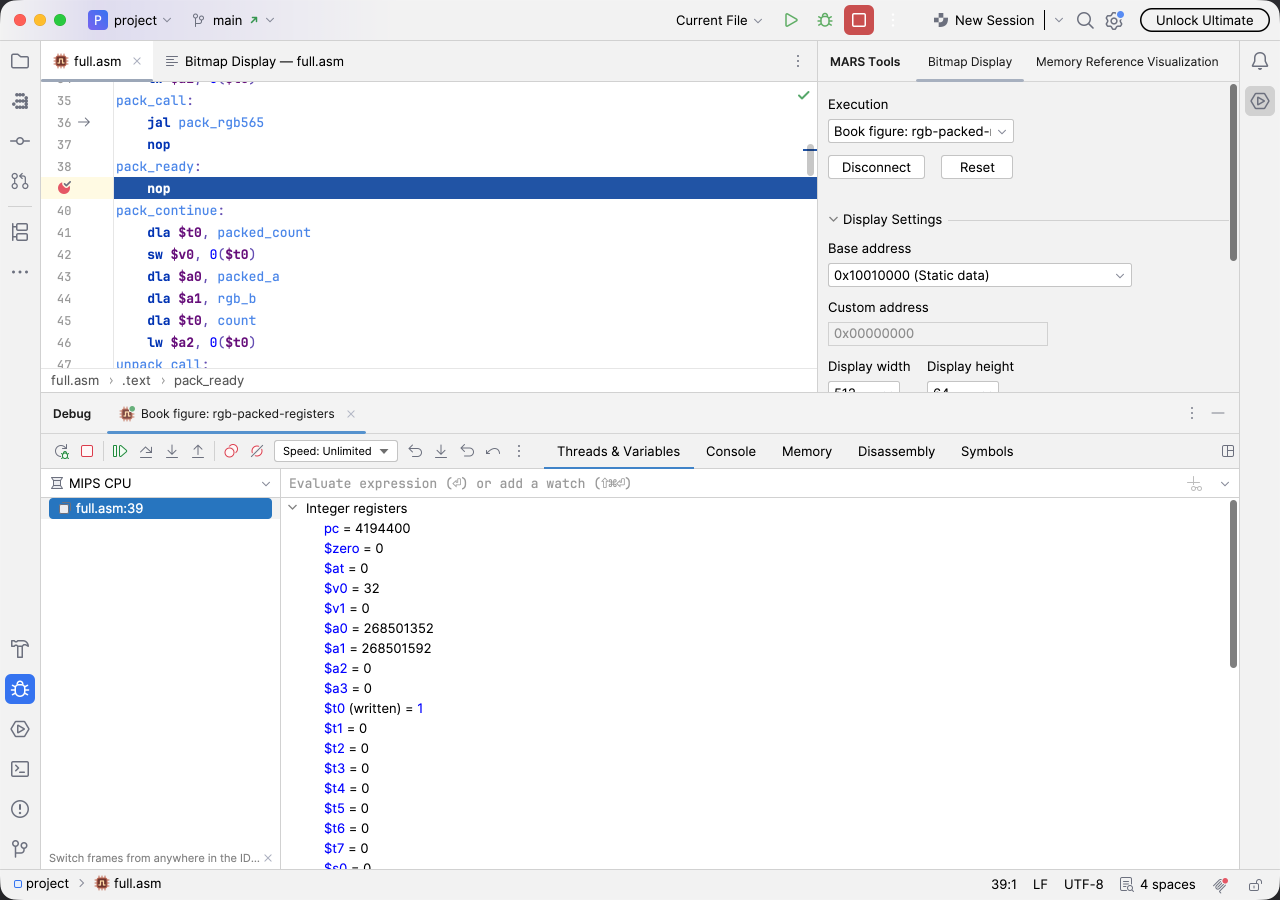
\includegraphics[artifact]{book/captures/019-rgb-formats/f01/registers.png}}
\sbox2{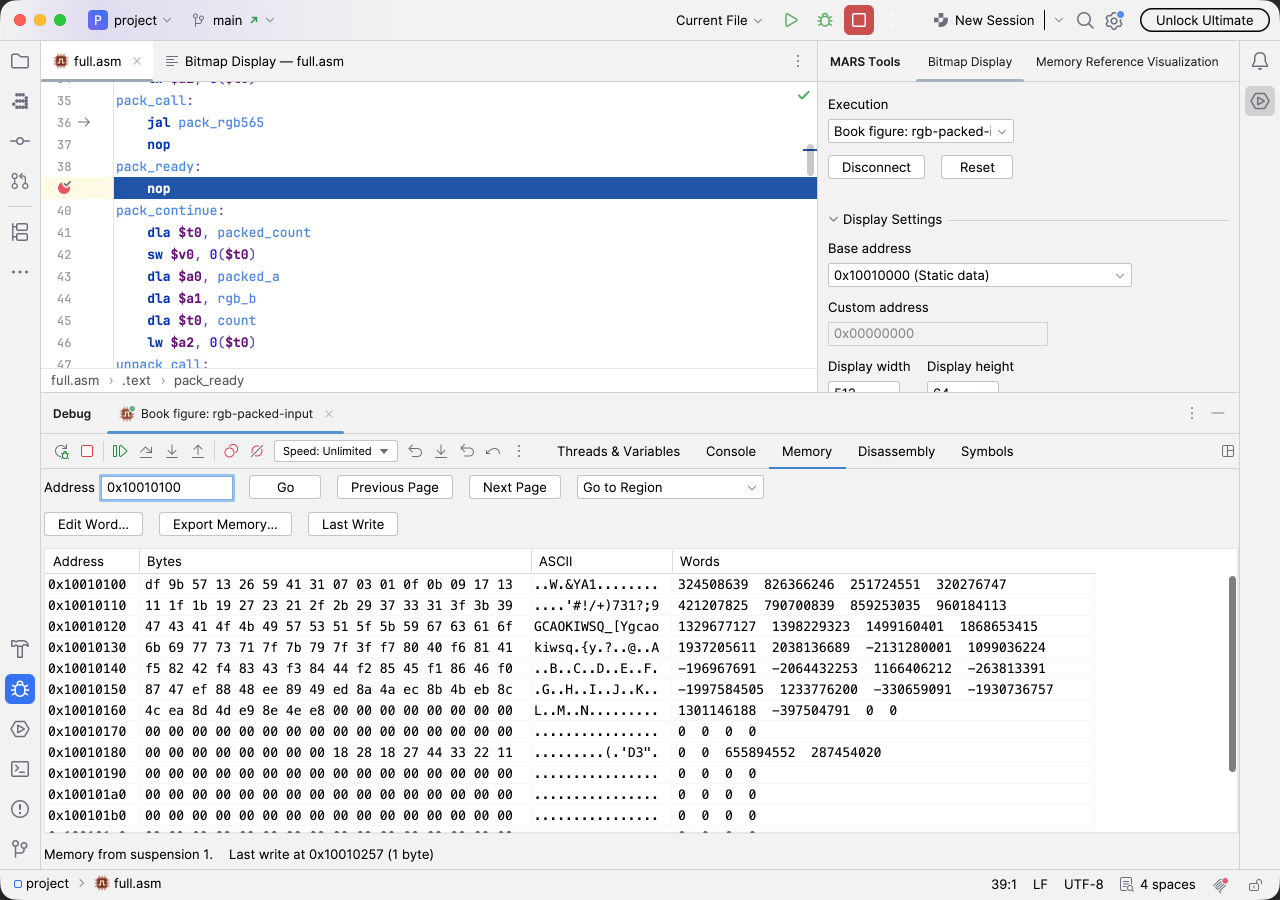
\includegraphics[artifact]{book/captures/019-rgb-formats/f01/input.png}}
\sbox4{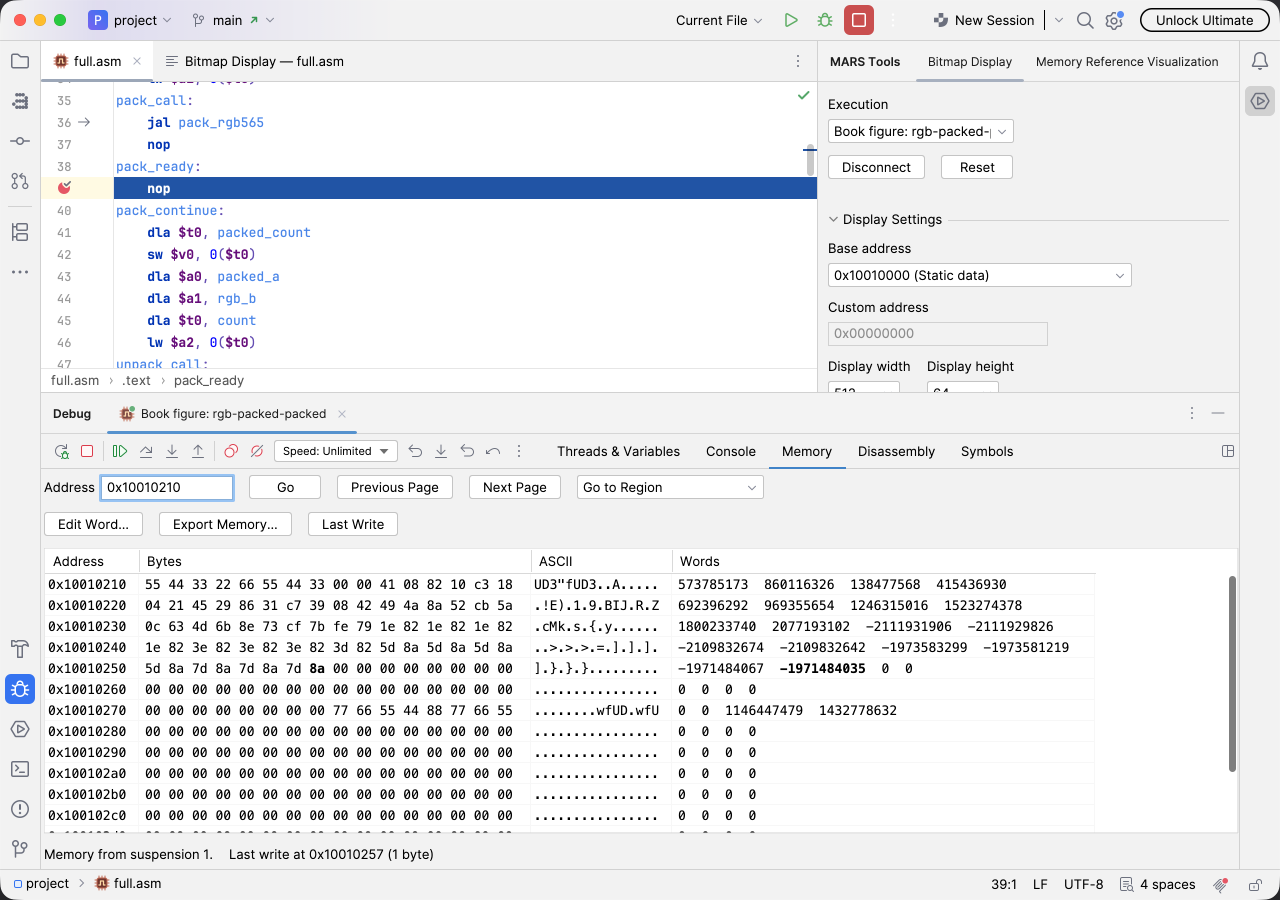
\includegraphics[artifact]{book/captures/019-rgb-formats/f01/packed.png}}
\sbox6{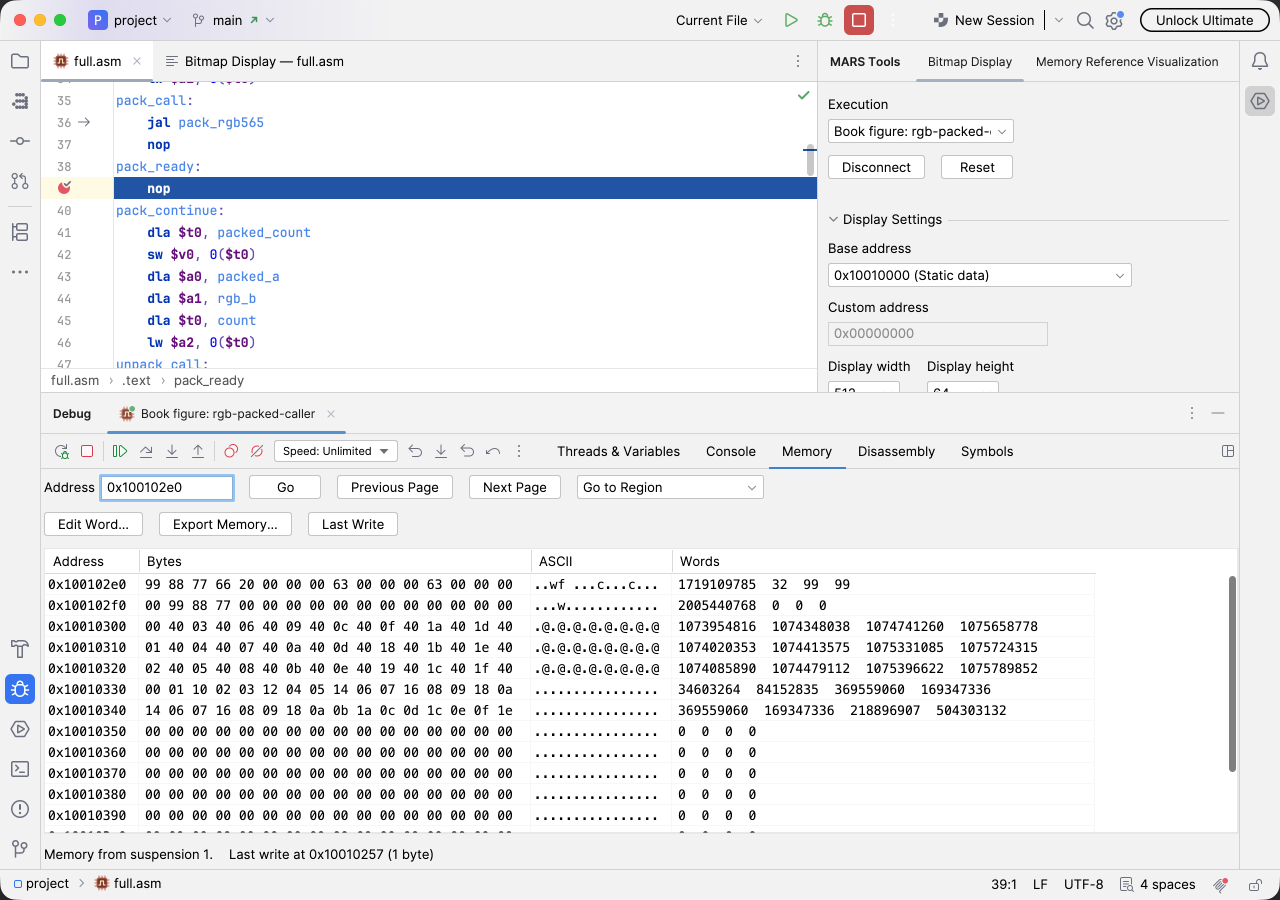
\includegraphics[artifact]{book/captures/019-rgb-formats/f01/caller.png}}
\edef\MARSrgbpackedsourceLeft{\the\dimexpr0.036718750\wd0\relax}
\edef\MARSrgbpackedsourceBottom{\the\dimexpr0.774444444\ht0\relax}
\edef\MARSrgbpackedsourceRight{\the\dimexpr0.713281250\wd0\relax}
\edef\MARSrgbpackedsourceTop{\the\dimexpr0.170000000\ht0\relax}
\edef\MARSrgbpackedregistersLeft{\the\dimexpr0.246093750\wd0\relax}
\edef\MARSrgbpackedregistersBottom{\the\dimexpr0.334444444\ht0\relax}
\edef\MARSrgbpackedregistersRight{\the\dimexpr0.553906250\wd0\relax}
\edef\MARSrgbpackedregistersTop{\the\dimexpr0.640000000\ht0\relax}
\edef\MARSrgbpackedinputLeft{\the\dimexpr0.034375000\wd2\relax}
\edef\MARSrgbpackedinputBottom{\the\dimexpr0.311111111\ht2\relax}
\edef\MARSrgbpackedinputRight{\the\dimexpr0.584375000\wd2\relax}
\edef\MARSrgbpackedinputTop{\the\dimexpr0.608888889\ht2\relax}
\edef\MARSrgbpackedpackedLeft{\the\dimexpr0.034375000\wd4\relax}
\edef\MARSrgbpackedpackedBottom{\the\dimexpr0.311111111\ht4\relax}
\edef\MARSrgbpackedpackedRight{\the\dimexpr0.584375000\wd4\relax}
\edef\MARSrgbpackedpackedTop{\the\dimexpr0.608888889\ht4\relax}
\edef\MARSrgbpackedcallerLeft{\the\dimexpr0.034375000\wd6\relax}
\edef\MARSrgbpackedcallerBottom{\the\dimexpr0.334444444\ht6\relax}
\edef\MARSrgbpackedcallerRight{\the\dimexpr0.584375000\wd6\relax}
\edef\MARSrgbpackedcallerTop{\the\dimexpr0.608888889\ht6\relax}
\begin{tikzpicture}[alt={Five annotated panels at pack_ready show returned pixel count 32, unchanged RGB source bytes, packed low-byte-first RGB565 and caller count fields 32, 99, 99. The first RGB triple seven, three, one quantizes to zero; the second fifteen, eleven, nine quantizes to hexadecimal 0841 stored as 41 08. Expanded and display buffers are still zero.}]
\node[anchor=north west,inner sep=0,font=\small\bfseries] (source-title) at (6mm,0) {Next instruction at this boundary};
\node[anchor=north west,inner sep=0] (source) at ([yshift=-1mm]source-title.south west) {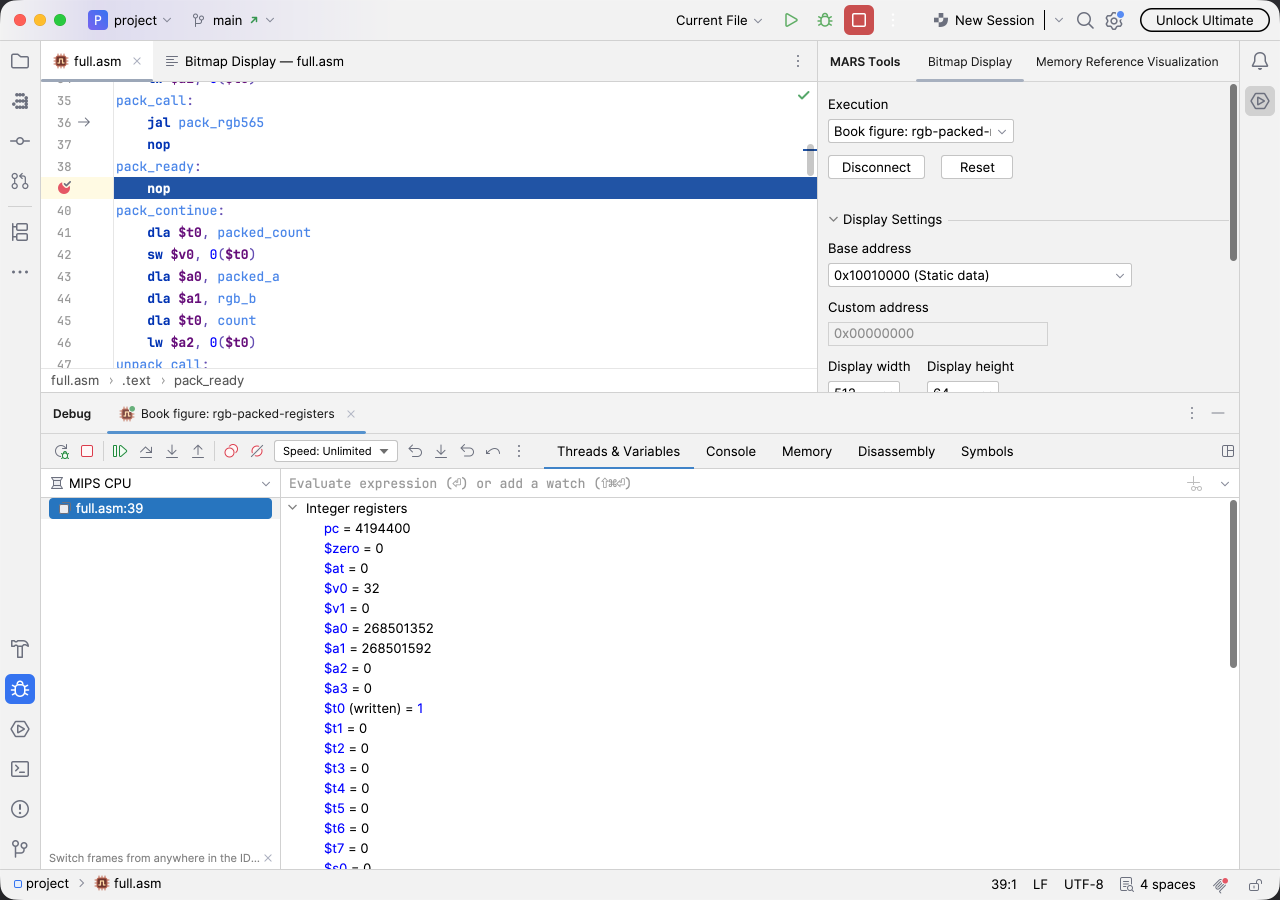
\includegraphics[width=0.54\linewidth,artifact,trim={\MARSrgbpackedsourceLeft{} \MARSrgbpackedsourceBottom{} \MARSrgbpackedsourceRight{} \MARSrgbpackedsourceTop{}},clip]{book/captures/019-rgb-formats/f01/registers.png}};
\begin{scope}[shift={(source.south west)},x={($(source.south east)-(source.south west)$)},y={($(source.north west)-(source.south west)$)}]
\draw[black,line width=0.7pt] (0.215625000,0.080000000) rectangle (0.384375000,0.520000000);
\node[draw=black,fill=white,circle,inner sep=1.5pt,font=\footnotesize] at ($(0.215625000,0.520000000)+(-3mm,0)$) {1};
\end{scope}
\node[anchor=north west,inner sep=0,font=\small\bfseries] (registers-title) at (0.58\linewidth,0 |- source-title.north) {Returned pixel count};
\node[anchor=north west,inner sep=0] (registers) at ([yshift=-1mm]registers-title.south west) {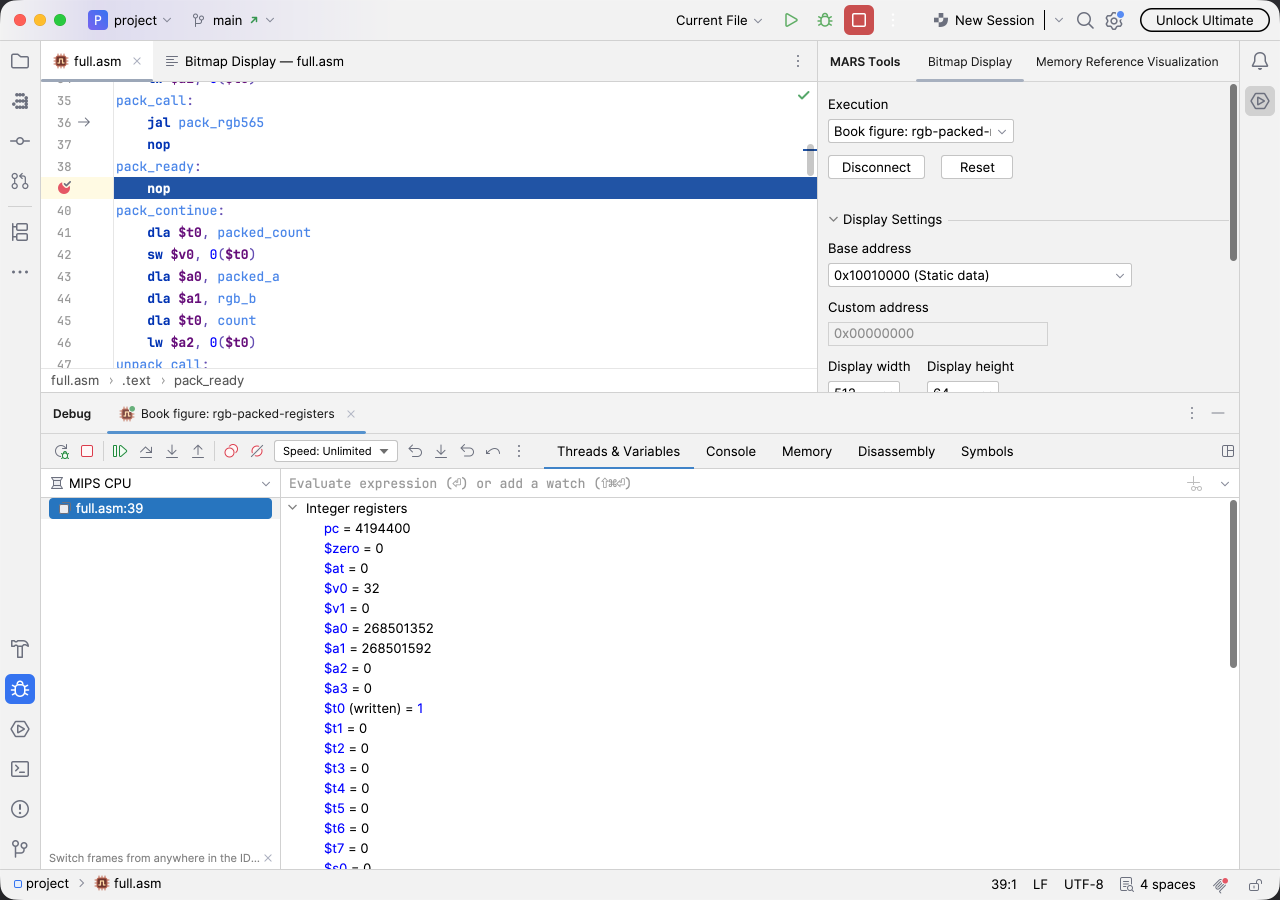
\includegraphics[width=0.42\linewidth,artifact,trim={\MARSrgbpackedregistersLeft{} \MARSrgbpackedregistersBottom{} \MARSrgbpackedregistersRight{} \MARSrgbpackedregistersTop{}},clip]{book/captures/019-rgb-formats/f01/registers.png}};
\begin{scope}[shift={(registers.south west)},x={($(registers.south east)-(registers.south west)$)},y={($(registers.north west)-(registers.south west)$)}]
\draw[black,line width=0.7pt] (0.023437500,0.043478261) rectangle (0.257812500,0.913043478);
\node[draw=black,fill=white,circle,inner sep=1.5pt,font=\footnotesize] at ($(0.023437500,0.913043478)+(-3mm,0)$) {2};
\end{scope}
\node[anchor=north west,inner sep=0,font=\small\bfseries] (input-title) at ([yshift=-1mm]source.south west) {Original RGB component bytes};
\node[anchor=north west,inner sep=0] (input) at ([yshift=-1mm]input-title.south west) {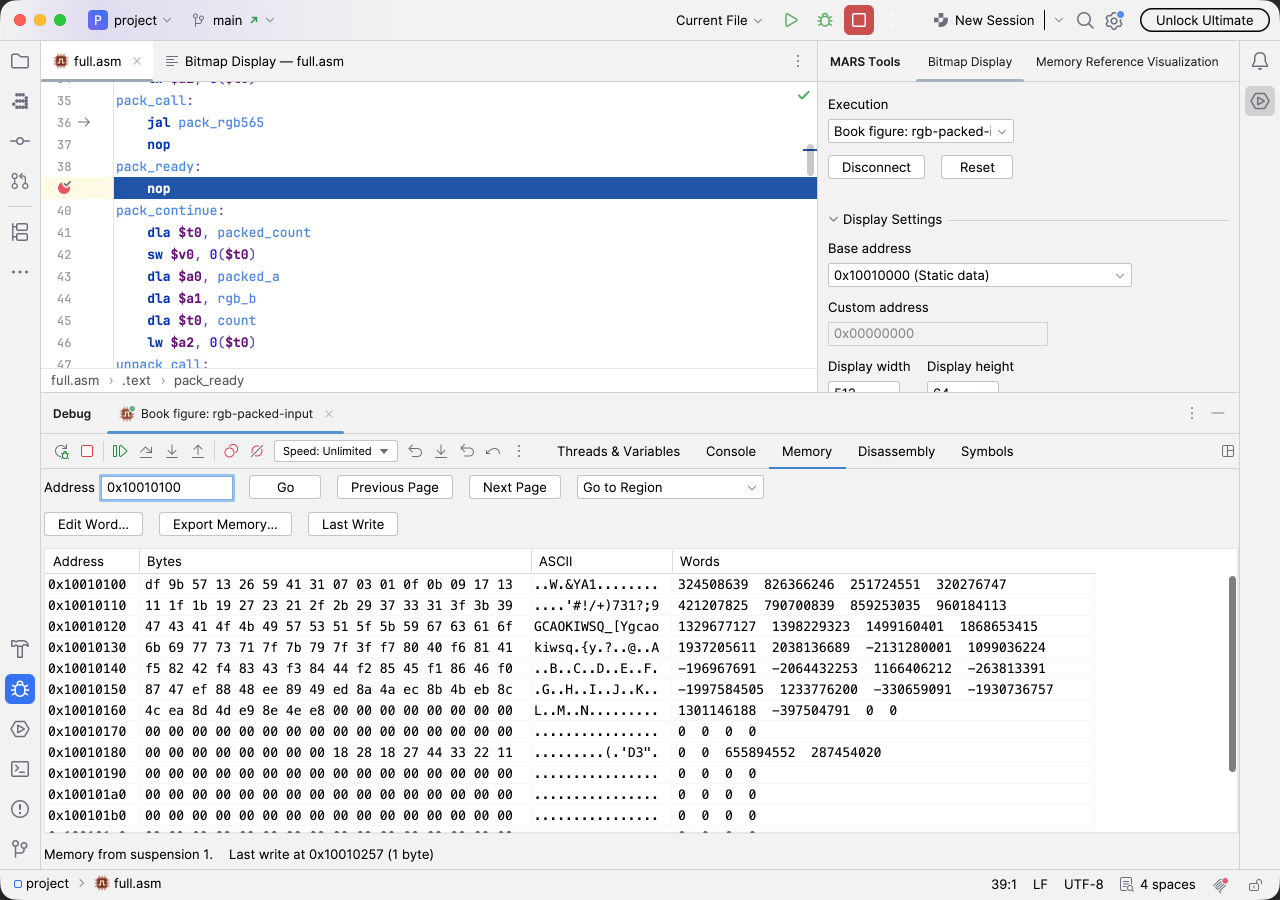
\includegraphics[width=0.84\linewidth,artifact,trim={\MARSrgbpackedinputLeft{} \MARSrgbpackedinputBottom{} \MARSrgbpackedinputRight{} \MARSrgbpackedinputTop{}},clip]{book/captures/019-rgb-formats/f01/input.png}};
\begin{scope}[shift={(input.south west)},x={($(input.south east)-(input.south west)$)},y={($(input.north west)-(input.south west)$)}]
\draw[black,line width=0.7pt] (0.194672131,0.055555556) rectangle (0.997950820,0.638888889);
\node[draw=black,fill=white,circle,inner sep=1.5pt,font=\footnotesize] at ($(0,0.638888889)+(-3mm,0)$) {3};
\end{scope}
\node[anchor=north west,inner sep=0,font=\small\bfseries] (packed-title) at ([yshift=-1mm]input.south west) {Low-byte-first RGB565};
\node[anchor=north west,inner sep=0] (packed) at ([yshift=-1mm]packed-title.south west) {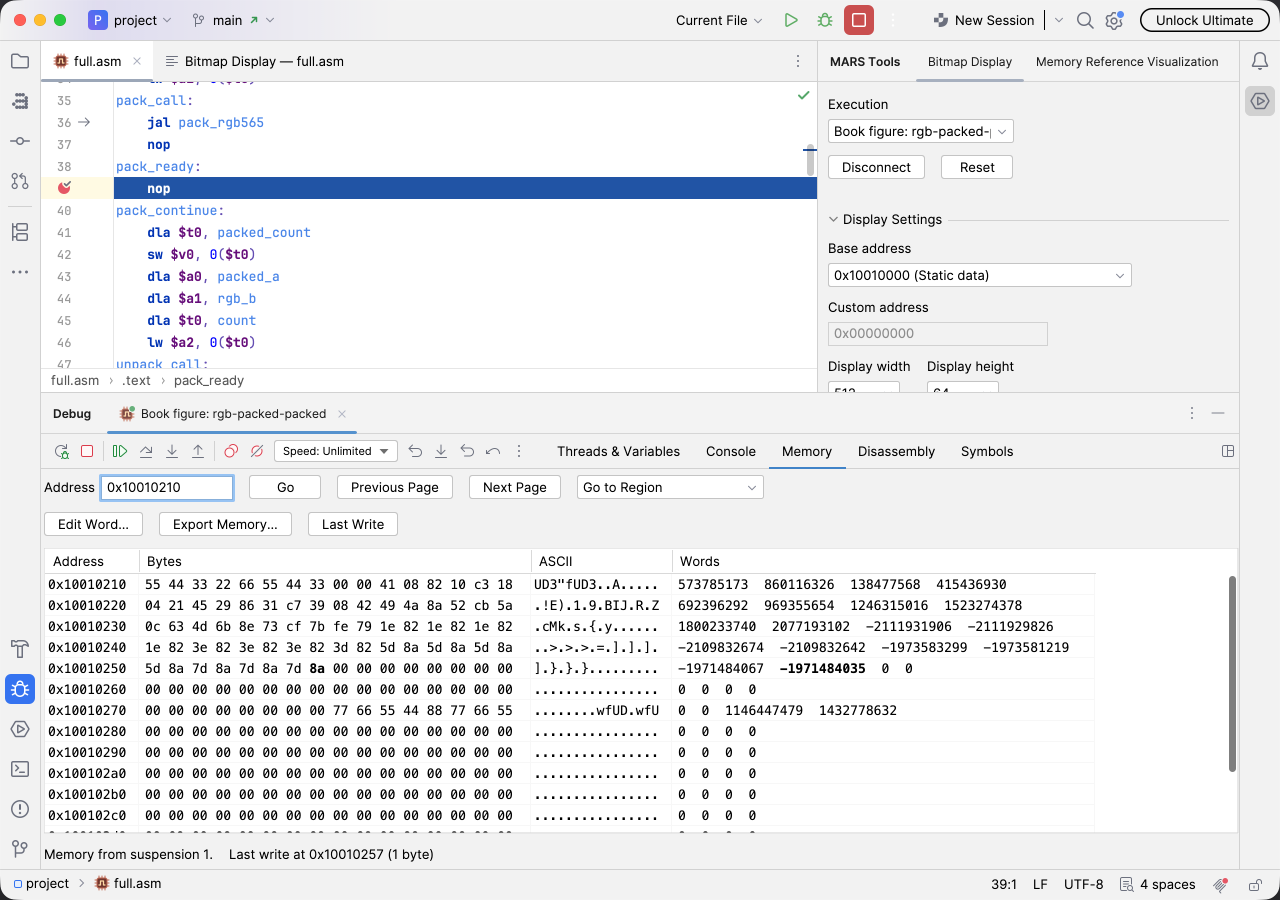
\includegraphics[width=0.84\linewidth,artifact,trim={\MARSrgbpackedpackedLeft{} \MARSrgbpackedpackedBottom{} \MARSrgbpackedpackedRight{} \MARSrgbpackedpackedTop{}},clip]{book/captures/019-rgb-formats/f01/packed.png}};
\begin{scope}[shift={(packed.south west)},x={($(packed.south east)-(packed.south west)$)},y={($(packed.north west)-(packed.south west)$)}]
\draw[black,line width=0.7pt] (0.194672131,0.055555556) rectangle (0.997950820,0.638888889);
\node[draw=black,fill=white,circle,inner sep=1.5pt,font=\footnotesize] at ($(0,0.638888889)+(-3mm,0)$) {4};
\end{scope}
\node[anchor=north west,inner sep=0,font=\small\bfseries] (caller-title) at ([yshift=-1mm]packed.south west) {Count and caller result words};
\node[anchor=north west,inner sep=0] (caller) at ([yshift=-1mm]caller-title.south west) {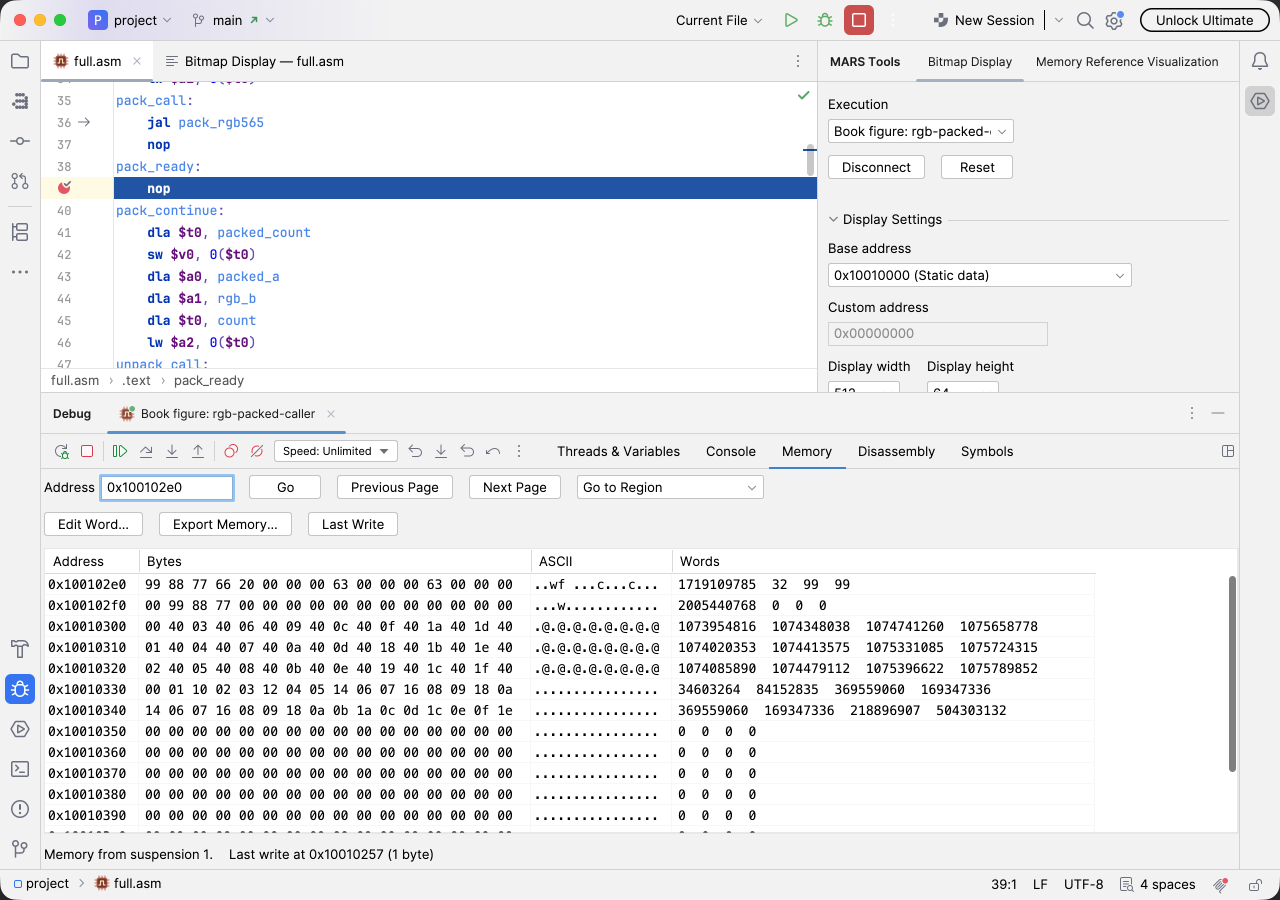
\includegraphics[width=0.84\linewidth,artifact,trim={\MARSrgbpackedcallerLeft{} \MARSrgbpackedcallerBottom{} \MARSrgbpackedcallerRight{} \MARSrgbpackedcallerTop{}},clip]{book/captures/019-rgb-formats/f01/caller.png}};
\begin{scope}[shift={(caller.south west)},x={($(caller.south east)-(caller.south west)$)},y={($(caller.north west)-(caller.south west)$)}]
\draw[black,line width=0.7pt] (0.194672131,0.078431373) rectangle (0.997950820,0.490196078);
\node[draw=black,fill=white,circle,inner sep=1.5pt,font=\footnotesize] at ($(0,0.490196078)+(-3mm,0)$) {5};
\end{scope}
\end{tikzpicture}
\par\smallskip
\begin{minipage}{\linewidth}
\small
\begin{enumerate}
\setlength{\itemsep}{2pt}
\setlength{\parsep}{0pt}
\item The blue \texttt{nop} at \texttt{pack\_ready} follows the packing return. Packed bytes are ready; the caller\textquotesingle s \texttt{packed\_count} store is still ahead. Expansion and preview construction have not executed.
\item \texttt{\$v0 = 32} counts pixels. Packing consumed 96 RGB bytes and produced 64 RGB565 bytes. The guided loop handles four groups of eight pixels; the public result reports the original count rather than bytes or groups.
\item RGB starts at \texttt{0x10010108}, after two guard words in the first shown row. The first triple is \texttt{07 03 01}. Every retained component is zero after discarding its low bits, so this nonzero input selects packed black.
\item Packed output starts at \texttt{0x10010218}. Its first pixel is \texttt{00 00}. The next input, $(15,11,9)$, retains fields $(1,2,1)$ and selects \texttt{0x0841}, stored as \texttt{41 08}. Byte order follows the format\textquotesingle s explicit low-byte-first rule.
\item The caller row contains a preceding guard, count 32, packed result 99 and expanded result 99. Those sentinels describe caller publication, not conversion progress. Complete memory checks confirm that expanded bytes, preview words, input and guards remain unchanged.
\end{enumerate}
\end{minipage}
\caption{Packing produces low-byte-first RGB565 before the caller stores its result.}
\label{capture:019-rgb-formats-f01}
\label{rgb-f01}
\end{figure}
\par
